
In this section we cover the basic definitions of foliations, and introduce some
of their local and global invariants, before looking at their behaviour under
blowups. Everything will be considered over $\C$.

\subsection{Foliations}

Suppose $X$ is a normal surface. To give a foliation $\scrF$ of $X$, we want to
define the tangent direction of the leaves of the foliation at any point in $X$,
giving a tangent vector up to scale at every point. We can accomplish this by
taking vector fields $v_i\in H^0(U_i,T_X)$ for an open cover $X=\cup_iU_i$, such
that $v_j=f_{ij}v_i$ for some non-vanishing holomorphic function
$f_{ij}\in H^0(U_i\cap U_j,\O_X^\times)$. Identifying data which would give rise
to the same foliation, we see that $\scrF$ is uniquely determined by the class
$\{f_{ij}\}$ in \v{C}ech cohomology $H^1(X,\O_X^\times)$, defining a line bundle
$T_\scrF$, and the global section $\{v_i\}$ of $T_\scrF^\vee\otimes T_X$ up to
multiplication by a nowhere vanishing holomorphic function.

\begin{example}
    Consider foliating $\A^2$ with horizontal leaves. The tangent direction for
    the leaves is generated by $\pdv{}{x}$, so $T_\scrF$ is trivial (as it must
    be on $\A^2$) with the section of $T_\scrF^\vee\otimes T_{\A^2}=T_{\A^2}$ given
    by $\pdv{}{x}$. Replacing $\pdv{}{x}$ by $-\pdv{}{x}$ or $2\pdv{}{x}$
    defines the same foliation.
    \begin{figure}[H]
        \centering
        
\begin{tikzpicture}
            \foreach \y in {-4,...,4}
                \draw (-4,\y*0.2) -- (4,\y*0.2);
        \end{tikzpicture}
        \caption{Foliation of $\A^2$ generated by $\pdv{}{x}$.}
    \end{figure}
\end{example}

We can also characterize the tangent spaces to the leaves as kernels of 1-forms,
leading to a similar definition with $T_X$ replaced by $\Omega^1_X$. The
foliation is given by a line bundle $N_\scrF^\vee$ and a global section
$\{\omega_i\}$ of $N_\scrF\otimes\Omega^1_X$ up to multiplication by a nowhere
vanishing holomorphic function.

\begin{example}
    The tangent vector $\pdv{}{x}$ on $\A^2$ is annhilated by the 1-form $dy$,
    and so the foliation from the previous example can also be seen as given by
    the trivial bundle $N_\scrF$ and the section $dy$ of
    $N_\scrF\otimes\Omega^1_{\A^2}$. We could construct $dy$ here by contracting
    $\pdv{}{x}$ with the area form $dx\wedge dy$, and so more generally the
    foliation generated by the vector field $A\pdv{}{x}+B\pdv{}{y}$ could also
    be specified by the contracted 1-form $Bdy-Adx$.
\end{example}

For a smooth foliation the tangent bundle $T_\scrF$ should be locally free, so
we would require that the vector fields $\{v_i\}$ (or the 1-forms
$\{\omega_i\}$) be non-vanishing. This is quite restrictive, and so in practice
we will be interested in foliations with singularities. We can also view the
above definitions as giving rational sections of $T_X$ or $\Omega^1_X$, defining
a global section after twisting by $\O(D)$ for $D$ a suitable divisor of poles.
There is a unique choice of $D$ such that the resulting section vanishes only in
codimension 2, and so we restrict our attention to foliations with singularities
in codimension 2.

\begin{example}\label{ex:parallel}
    Consider the extension of the foliation generated by $\pdv{}{x}$ on $\A^2$
    to $\P^2$. In coordinates $[1:y:z]$ the 1-form $dy$ on $\A^2$ becomes
    $d(y/z)=dy/z-ydz/z^2$, with a pole of order 2 along the hyperplane at
    infinity. Hence we get a section $(zdy-ydz)/z^2$ of $\Omega^1_{\P^1}(2)$
    which vanishes at $[1:0:0]\in\P^2$, defining a foliation $\scrF$ with
    $N_\scrF=\O(2)$ and a singularity at $[1:0:0]$. Note that the local form of
    the singularity is generated by the radial vector field
    $y\pdv{}{y}+z\pdv{}{z}$ annhilated by $zdy-ydz$, illustrated in
    \cref{fig:parallel}.
    \begin{figure}[H]
        \centering
        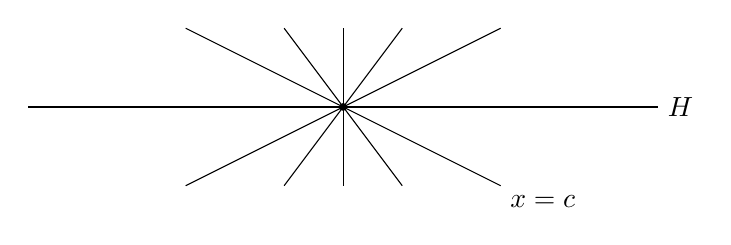
\begin{tikzpicture}
            \draw (-4,0)
                -- (0,0) node[circle,fill,inner sep=1pt] {}
                -- (4,0) node[anchor=west] {$H$};
            \draw (0,1) -- (0,-1);
            \draw (-0.75,-1) -- (0.75,1);
            \draw (0.75,-1) -- (-0.75,1);
            \draw (-2,-1) -- (2,1);
            \draw (2,-1) node[anchor=north west] {$x=c$} -- (-2,1);
        \end{tikzpicture}
        \caption{Parallel leaves converging at the horizon.}
        \label{fig:parallel}
    \end{figure}
\end{example}

The perspective of a foliation as the subsheaf $T_\scrF$ in $T_X$ leads us to a
general definition of foliations for higher dimensions.

\begin{definition}\label{defn:foliation}
    A rank $r$ foliation $\scrF$ of a normal variety $X$ is a rank $r$ subsheaf
    $T_\scrF$ of $T_X$ such that
    \begin{enumerate}[label=\roman*.]
        \item $T_X/T_\scrF$ is torsion-free,
        \item $T_\scrF$ is closed under the Lie bracket on $T_X$.
    \end{enumerate}
    The singular locus $\Sing(\scrF)$ is the singular locus of $X$ together with
    the locus where the stalks of $T_\scrF$ are not locally free submodules of
    the stalks of $T_X$.
\end{definition}

\begin{remark}
    Note that ii. is automatically satisfied for rank 1 foliations, as the Lie
    bracket then vanishes on $T_\scrF$. This condition is the requirement for
    integrability, leading to \cref{thm:frobenius}.
\end{remark}

See \cite[\S2]{friedman_book} for properties of torsion-free sheaves and
singularities of coherent sheaves. It follows that $T_X/T_\scrF$ is a subsheaf
of a locally free sheaf of the same rank, so in the case of a rank 1 foliation
on a surface we get $T_X/T_\scrF=I\cdot N_\scrF$ where $N_\scrF$ is a line
bundle and $I$ is the ideal sheaf cutting out $\Sing(\scrF)$. We then have two
dual exact sequences
\begin{equation}\label{eqn:tangent sequence}
    0 \to T_\scrF \to T_X \to I\cdot N_\scrF \to 0
\end{equation}
and
\begin{equation}\label{eqn:1-form sequence}
    0 \to N_\scrF^\vee \to \Omega^1_X \to I\cdot T_\scrF^\vee \to 0.
\end{equation}
Of course, the 1-forms vanishing on $T_\scrF$ are dual to $T_X/T_\scrF$,
justifying the re-use of the name $N_\scrF$ from above. The inclusion
$N_\scrF^\vee\to\Omega^1_X$ is given by the section of $N_\scrF\otimes\Omega^1_X$
defining the foliation.

\begin{remark}
    Since a foliation is specified by an (almost) non-vanishing vector field up
    to scale, we can view it as an (almost) section of the projective tangent
    bundle $\P(T_X)\to X$, i.e. a rational section with domain of definition the
    complement of $\Sing(\scrF)$. Similarly, the 1-form perspective gives a
    rational section of the projective cotangent bundle $\P(\Omega^1_X)\to X$.
    The fact that these are equivalent can be seen from the fact that
    $\Omega^1_X=T_X\otimes K_X$, giving an isomorphism $\P(\Omega^1_X)=\P(T_X)$.
    See \cite[\nopp II]{mcquillan_98} for more context. This will come up in
    \cref{sec:stability}.
\end{remark}

We now restrict our attention to the case of a rank 1 foliation $\scrF$ on a
surface $X$.

\begin{proposition}\label{prop:canonical}
    $K_X=T_\scrF^\vee\otimes N_\scrF^\vee$.
\end{proposition}

\begin{proof}
    Non-vanishing sections of $K_X$ give by contraction an isomorphism between
    vector fields and 1-forms, identifying $T_\scrF$ and $N_\scrF^\vee$. In this
    way we get an isomorphism
    $K_X=\shHom(T_\scrF,N_\scrF^\vee)=T_\scrF^\vee\otimes N_\scrF^\vee$. This can also be
    seen from the exact sequence \cref{eqn:1-form sequence}, which restricts to
    an exact sequence of vector bundles on $U=X\setminus\Sing(\scrF)$, giving
    $K_X|_U=(N_\scrF^\vee\otimes T_\scrF^\vee)|_U$ by taking determinants, which
    implies the result because $\Sing(\scrF)$ has codimension at least 2.
\end{proof}

\begin{example}\label{ex:P2 tangent}
    In the example of $\pdv{}{x}$ extended to $\P^2$ we had $N_\scrF=\O(2)$.
    Since $K_{\P^2}=\O(-3)$, the proposition gives $T_\scrF=\O(1)$, so
    $\pdv{}{x}$ should extend to a section of $T_{\P^2}(-1)$. Indeed in
    coordinates $[1:y:z]$ the pushforward of $\pdv{}{x}$ is
    $-z(y\pdv{}{y}+z\pdv{}{z})$, vanishing to first order at infinity.
\end{example}

\begin{definition}
    The \emph{canonical bundle} of the foliation $\scrF$ is
    $K_\scrF\coloneqq K_X\otimes N_\scrF=T_\scrF^\vee$.
\end{definition}

\begin{example}
    In the previous example $T_\scrF=\O(1)$, so $K_\scrF=\O(-1)$.
\end{example}

\subsection{Invariant curves}

To relate a foliation defined by a vector field or 1-form to the intuitive
notion of leaves foliating a surface, we have to consider its integral curves,
which give the leaves of the foliation. In general, the solutions to the
relevant differential equation will be analytic but not algebraic.

\begin{definition}
    If $(X,\scrF)$ is a foliated surface, a holomorphic curve $C$ in $X$ is
    \emph{invariant} under $\scrF$ if the map $T_C\to T_X$ factors through
    $T_\scrF$.
\end{definition}

\begin{example}\label{ex:irrational}
    Consider the foliation of $\A^2$ generated by $xdy+\sqrt2ydx$, corresponding
    to $x\pdv{}{x}-\sqrt2y\pdv{}{y}$. The differential equations defining an
    invariant curve are
    \begin{equation*}
        \dot x(t) = x(t), \quad \dot y(y)=-\sqrt2y(t).
    \end{equation*}
    There are two algebraic curves $\{x=0\}$ and $\{y=0\}$ which are invariant,
    and away from them the equations can be integrated to an analytic
    parametrization $x(t)=x_0e^t$, $y(t)=y_0e^{-\sqrt2t}$ defining local
    analytic curves $xy^{1/\sqrt2}=x_0y_0^{1/\sqrt2}$ which are \emph{not}
    algebraic. (Note that if we replace $\sqrt2$ with a rational number, e.g. 2,
    then a multiple of the resulting 1-form has an algebraic integral;
    $x(xdy+2ydx)=d(x^2y)$, and the leaves are algebraic; $x^2y=x_0^2y_0$.)
    \begin{figure}[H]
        \centering
        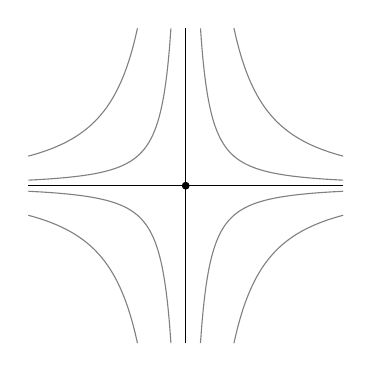
\begin{tikzpicture}
            \foreach \sx in {-0.5,0.5}
                \foreach \sy in {-0.5,0.5}
                    \draw[domain=-0.98:1.386, color=gray, smooth, variable=\t]
                        plot ({\sx*exp(\t)}, {\sy*exp(-sqrt(2)*\t)});
            \foreach \sx in {-1,1}
                \foreach \sy in {-1,1}
                    \draw[domain=-0.49:0.693, color=gray, smooth, variable=\t]
                        plot ({\sx*exp(\t)}, {\sy*exp(-sqrt(2)*\t)});
            \draw (-2,0) -- (2,0);
            \draw (0,-2) -- (0,2);
            \node[circle, fill, inner sep=1pt] at (0,0) {};
        \end{tikzpicture}
        \caption{Leaves of $xdy+\sqrt{2}ydx$.}
        \label{fig:irrational}
    \end{figure}
\end{example}

In fact, we have the following theorem (cf. \cite[Thm 2.20]{voisin_book}).

\begin{theorem}[Frobenius]\label{thm:frobenius}
    If $X$ is a smooth complex analytic variety, and $\scrF$ is a foliation on
    $X$, then for any $x\in X\setminus\Sing(\scrF)$ there is an analytic
    neighbourhood $U$ of $x$ and a holomorphic submersion $F:U\to W\subset\C^r$
    such that $T_\scrF|_U=\ker(dF)$.
\end{theorem}

Hence near smooth points we always have locally defined analytic leaves, given
as the fibers of a holomorphic submersion. In particular, invariant curves can
only intersect at singularities of the foliation. A key result for the local
structure at singular points is the ``separatrix theorem''.

\begin{definition}
    A \emph{separatrix} at $p\in\Sing(\scrF)$ is a local holomorphic curve $C$
    passing through $p$ and invariant under $\scrF$.
\end{definition}

\begin{theorem}[Camacho--Sad, \cite{camacho_sad_82}]\label{thm:separatrix}
    If $X$ is a smooth surface, with foliation $\scrF$, then through every
    $p\in\Sing(\scrF)$ there exists at least one separatrix.
\end{theorem}

In fact there are generalizations of this result to the case of singular $X$;
see \cite{camacho_88}.

\begin{example}
    In \cref{ex:irrational} we found two separatrices: $\{x=0\}$ and
    $\{y=0\}$.
\end{example}

\begin{remark}
    As a consequence of \cref{thm:frobenius}, if two invariant curves intersect
    (or if an invariant curve has a node), then the intersection point is a
    singularity of the foliation.
\end{remark}

It is worth noting that while the leaves of the foliation can always be locally
defined by an analytic equation, the global geometry can be quite pathalogical.
Take the foliation from \cref{ex:irrational}. It is hard to visualize the global
geometry of the leaves for dimension reasons, but we can intersect with the
torus $S^1\times S^1\subset\C^2$. The slices in $S^1\times S^1$ of the leaves of
$\scrF$ are parametrized as $x(t)=e^{it}$, $y(t)=e^{\phi-i\sqrt2t}$ for
$t\in\R$, where $\phi\in\R$ is fixed for each leaf. We recover the classical
example of a pathalogical immersion of $\R$ in the torus; each leaf is not just
Zariski dense, but classically dense. This highlights one of the dangers of
relying on pictures like \cref{fig:irrational} depicting only the real locus.

\begin{figure}[H]
    \centering
    \begin{tikzpicture}
        \draw[color=gray] (0.414,-1.000) -- (1,-0.172);
        \draw[color=gray] (-1.000,-0.172) -- (-0.172,1);
        \draw[color=gray] (-0.172,-1.000) -- (1,0.657);
        \draw[color=gray] (-1.000,0.657) -- (-0.757,1);
        \draw[color=gray] (-0.757,-1.000) -- (0.657,1);
        \draw[color=gray] (0.657,-1.000) -- (1,-0.515);
        \draw[color=gray] (-1.000,-0.515) -- (0.071,1);
        \draw[color=gray] (0.071,-1.000) -- (1,0.314);
        \draw[color=gray] (-1.000,0.314) -- (-0.515,1);
        \draw[color=gray] (-0.515,-1.000) -- (0.899,1);
        \draw[color=gray] (0.899,-1.000) -- (1,-0.858);
        \draw[color=gray] (-1.000,-0.858) -- (0.314,1);
        \draw[color=gray] (0.314,-1.000) -- (1,-0.029);
        \draw[color=gray] (-1.000,-0.029) -- (-0.272,1);
        \draw[color=gray] (-0.272,-1.000) -- (1,0.799);
        \draw[color=gray] (-1.000,0.799) -- (-0.858,1);
        \draw[color=gray] (-0.858,-1.000) -- (0.556,1);
        \draw[color=gray] (0.556,-1.000) -- (1,-0.373);
        \draw[color=gray] (-1.000,-0.373) -- (-0.029,1);

        \begin{scope}[very thick,decoration={
            markings,
            mark=at position 0.52 with {\arrow{>}}
        }]
            \draw[postaction={decorate}] (-1,-1) -- (-1,1);
            \draw[postaction={decorate}] (1,-1) -- (1,1);
        \end{scope}
        \begin{scope}[very thick,decoration={
            markings,
            mark=at position 0.57 with {\arrow{>>}}
        }]
            \draw[postaction={decorate}] (-1,-1) -- (1,-1);
            \draw[postaction={decorate}] (-1,1) -- (1,1);
        \end{scope}
    \end{tikzpicture}
    \caption{A slice of a single leaf of $xdy+\sqrt2ydx$.}
\end{figure}

\subsection{Singularities}

In view of \cref{thm:frobenius} the local picture of $\scrF$ at smooth points
is relatively simple, so we will be interested in the local theory of the
singular points. We will look at some invariants of the singularities of $\scrF$
which can be used to identify classes of ``nice'' singularities out of all the
possible modifications (under e.g. blowups) of a singularity, and can be
accumulated to provide some global information about $\scrF$. We will only
consider the case where the underlying surface is smooth.

\subsubsection{Multiplicity}

Fix a foliation $\scrF$ on a smooth surface $X$, with a singular point
$p\in\Sing(\scrF)$. Taking local analytic coordinates $x,y$ near $p=(0,0)$, we
have a generator $A\pdv{}{x}+B\pdv{}{y}$ for $\scrF$.

\begin{definition}
    The \emph{multiplicity} of the singularity $p$ is
    \begin{equation*}
        m(\scrF,p)\coloneqq\dim_\C\hat\O_{X,p}/(A,B).
    \end{equation*}
    We may then define a count of the total number of singularities of $\scrF$:
    \begin{equation*}
        m(\scrF) \coloneqq \sum_{p\in\Sing(\scrF)}m(\scrF,p),
    \end{equation*}
    which is a finite sum provided that $X$ is compact.
\end{definition}

\begin{remark}
    One could also view $m(\scrF,p)$ as the multiplicity at $p$ of the
    0-dimensional subscheme $\Sing(\scrF)\subset X$ cut out by the ideal sheaf
    in \cref{eqn:tangent sequence}.
\end{remark}

\begin{example}
    For the foliation given by $xdy+ydx$ a generating vector field is
    $x\pdv{}{x}-y\pdv{}{y}$, so the multiplicity at the origin is
    \begin{equation*}
        \dim_\C\C[x,y]/(x,y) = 1.
    \end{equation*}
    If we instead consider the foliation generated by $x\pdv{}{x}+y^2\pdv{}{y}$,
    then the multiplicity at the origin is
    \begin{equation*}
        \dim_\C\C[x,y]/(x,y^2) = 2.
    \end{equation*}
    Note that perturbing this to the foliation $x\pdv{}{x}+(y^2+\epsi)\pdv{}{y}$
    results in two singularities $(0,\pm\sqrt\epsi)$ both with multiplicity 1.
    \begin{figure}[H]
        \centering
        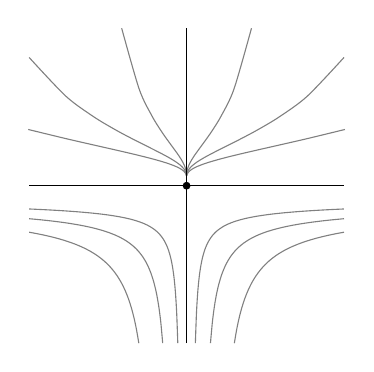
\begin{tikzpicture}
            % sy = 1
            \foreach \sx in {-0.5,0.5}
                \draw[domain=-7:0.5, color=gray, smooth, variable=\t]
                    plot ({\sx*exp(\t)}, {1/(1-\t)});
            \foreach \sx in {-3,3}
                \draw[domain=-7:-0.4, color=gray, smooth, variable=\t]
                    plot ({\sx*exp(\t)}, {1/(1-\t)});
            % sy = 0.5
            \foreach \sx in {-0.5,0.5}
                \draw[domain=-5:1.386, color=gray, smooth, variable=\t]
                    plot ({\sx*exp(\t)}, {1/(2-\t)});

            % sy = -0.5
            \foreach \sx in {-0.5,0.5}
                \draw[domain=-1.5:1.386, color=gray, smooth, variable=\t]
                    plot ({\sx*exp(\t)}, {-1/(2+\t)});
            % sy = -1
            \foreach \sx in {-0.5,0.5}
                \draw[domain=-0.5:1.386, color=gray, smooth, variable=\t]
                    plot ({\sx*exp(\t)}, {-1/(1+\t)});
            \foreach \sx in {-1,1}
                \draw[domain=-0.5:0.693, color=gray, smooth, variable=\t]
                    plot ({\sx*exp(\t)}, {-1/(1+\t)});

            \draw (-2,0) -- (2,0);
            \draw (0,-2) -- (0,2);
            \node[circle, fill, inner sep=1pt] at (0,0) {};
        \end{tikzpicture}
        \caption{The foliation generated by $x\pdv{}{x}+y^2\pdv{}{y}$.}
        \label{fig:saddle-node}
    \end{figure}
\end{example}

\begin{proposition}\label{prop:multiplicity}
    Suppose $(X,\scrF)$ is a compact foliated surface. Then
    \begin{align*}
        m(\scrF)
            = T_\scrF\cdot T_\scrF + T_\scrF\cdot K_X + c_2(X)
            = c_2(X) - T_\scrF\cdot N_\scrF.
    \end{align*}
\end{proposition}

\begin{proof}
    Note that the second equality is immediate from
    $K_\scrF=-T_\scrF=K_X+N_\scrF$, \cref{prop:canonical}. For the first
    equality, note that $c_2(T_\scrF^\vee\otimes T_X)$ is given by the vanishing
    locus of the section in $H^0(T_\scrF^\vee\otimes T_X)$ corresponding to the
    inclusion $T_\scrF\to T_X$, which has isolated zeros at the singularities of
    $\scrF$. The intersection multiplicity with the zero section at
    $p\in\Sing(\scrF)$ is precisely $m(\scrF,p)$, and so
    \begin{equation*}
        m(\scrF) = c_2(T_\scrF^\vee\otimes T_X).
    \end{equation*}
    Now recall that
    \begin{equation*}
        c_2(T_\scrF^\vee\otimes T_X)
            = c_2(T_X) + c_1(T_X)c_1(T_\scrF^\vee) + c_1(T_\scrF^\vee)^2,
    \end{equation*}
    which can be seen from the splitting principle:
    \begin{align*}
        c_2(L\otimes(L_1\oplus L_2))
            &= (c_1(L)+c_1(L_1))(c_1(L)+c_1(L_2)) \\
            &= c_1(L_1)c_1(L_2) + (c_1(L_1)+c_1(L_2))c_1(L) + c_1(L)^2 \\
            &= c_2(L_1\oplus L_2) + c_1(L_1\oplus L_2)c_1(L) + c_1(L)^2.
    \end{align*}
    The result then follows from $c_1(T_X)=-c_1(K_X)$,
    $c_1(T_\scrF^\vee)=-c_1(T_\scrF)$.
\end{proof}

\begin{example}
    Recall that the Chern character of $\P^n$ is $(1+h)^{n+1}$ for $h$ a
    hyperplane class, so the Euler class is $(n+1)h^n$. Hence $c_2(\P^2)=3$, so
    for a foliation of $\P^2$ we must have
    $m(\scrF)=3+T_\scrF\cdot T_\scrF+T_\scrF\cdot K_{\P^2}$. In
    \cref{ex:P2 tangent} we found $T_\scrF=\O(1)$, so
    \begin{equation*}
        m(\scrF) = 3 + H\cdot H + H\cdot(-3H) = 3 + 1 - 3 = 1.
    \end{equation*}
    Indeed, there was one singularity with the local form
    $y\pdv{}{y}+z\pdv{}{z}$, which has multiplicity 1. In fact the integer
    $T_\scrF\cdot T_\scrF+T_\scrF\cdot K_X$ must always be even, from
    computations with Stiefel--Whitney classes $w=\Sq(\nu)$ and their relation
    to the Wu and Chern classes (see \cite{milnor_book}, \S8 and \S14):
    \begin{align*}
        L\cdot K_X
            = -c_1(X)c_1(L)
            &\equiv w_2(X)w_2(L)
            & &\text{reducing mod 2} \\
            &\equiv (\nu_2(X)-w_1(X)^2)w_2(L)
            & &\text{from $w=\Sq(\nu)$} \\
            &\equiv \nu_2(X)w_2(L)
            & &\text{odd $w_k$ vanish} \\
            &\equiv w_2(L)^2 
            & &\text{from $\Sq^k(\alpha_k)=\alpha_k^2$} \\
            &\equiv c_1(L)^2 \mod2
    \end{align*}
    for any line bundle $L$. Hence a foliation of $\P^2$ must have an odd number
    of singularities, and in particular at least one.
\end{example}

\begin{remark}
    It can be shown directly that there is no exact sequence of the form
    $0\to\O(a)\to\Omega^1_{\P^2}\to\O(b)\to0$ on $\P^2$, so that there can be no
    smooth foliation, but this doesn't obviously generalize to a parity
    constraint.
\end{remark}

\subsubsection{Holonomy}

Now we consider the case of a separatrix $C$ through $p\in\Sing(\scrF)$. A
punctured neighbourhood of $p$ in $C$ is isomorphic to the punctured disc
$\D^*\subset\C$, and has fundamental group generated by a loop $\gamma$. We may
locally project the coordinates on $X$ to $C$, and given a lift of the base of
$\gamma$ we obtain a unique path lifting $\gamma$ in a neighbouring leaf of
$\scrF$. This lifted path may no longer be a loop, and so taking the endpoint
gives an endomorphism of the fiber of this projection over the basepoint.
Writing $D$ for this fiber, we have a homomorphism from
$\pi_1(C\setminus\{p\})\simeq\Z$ to (locally defined) biholomorphisms of $D$
relative to $p$.

\begin{figure}[H]
    \centering
    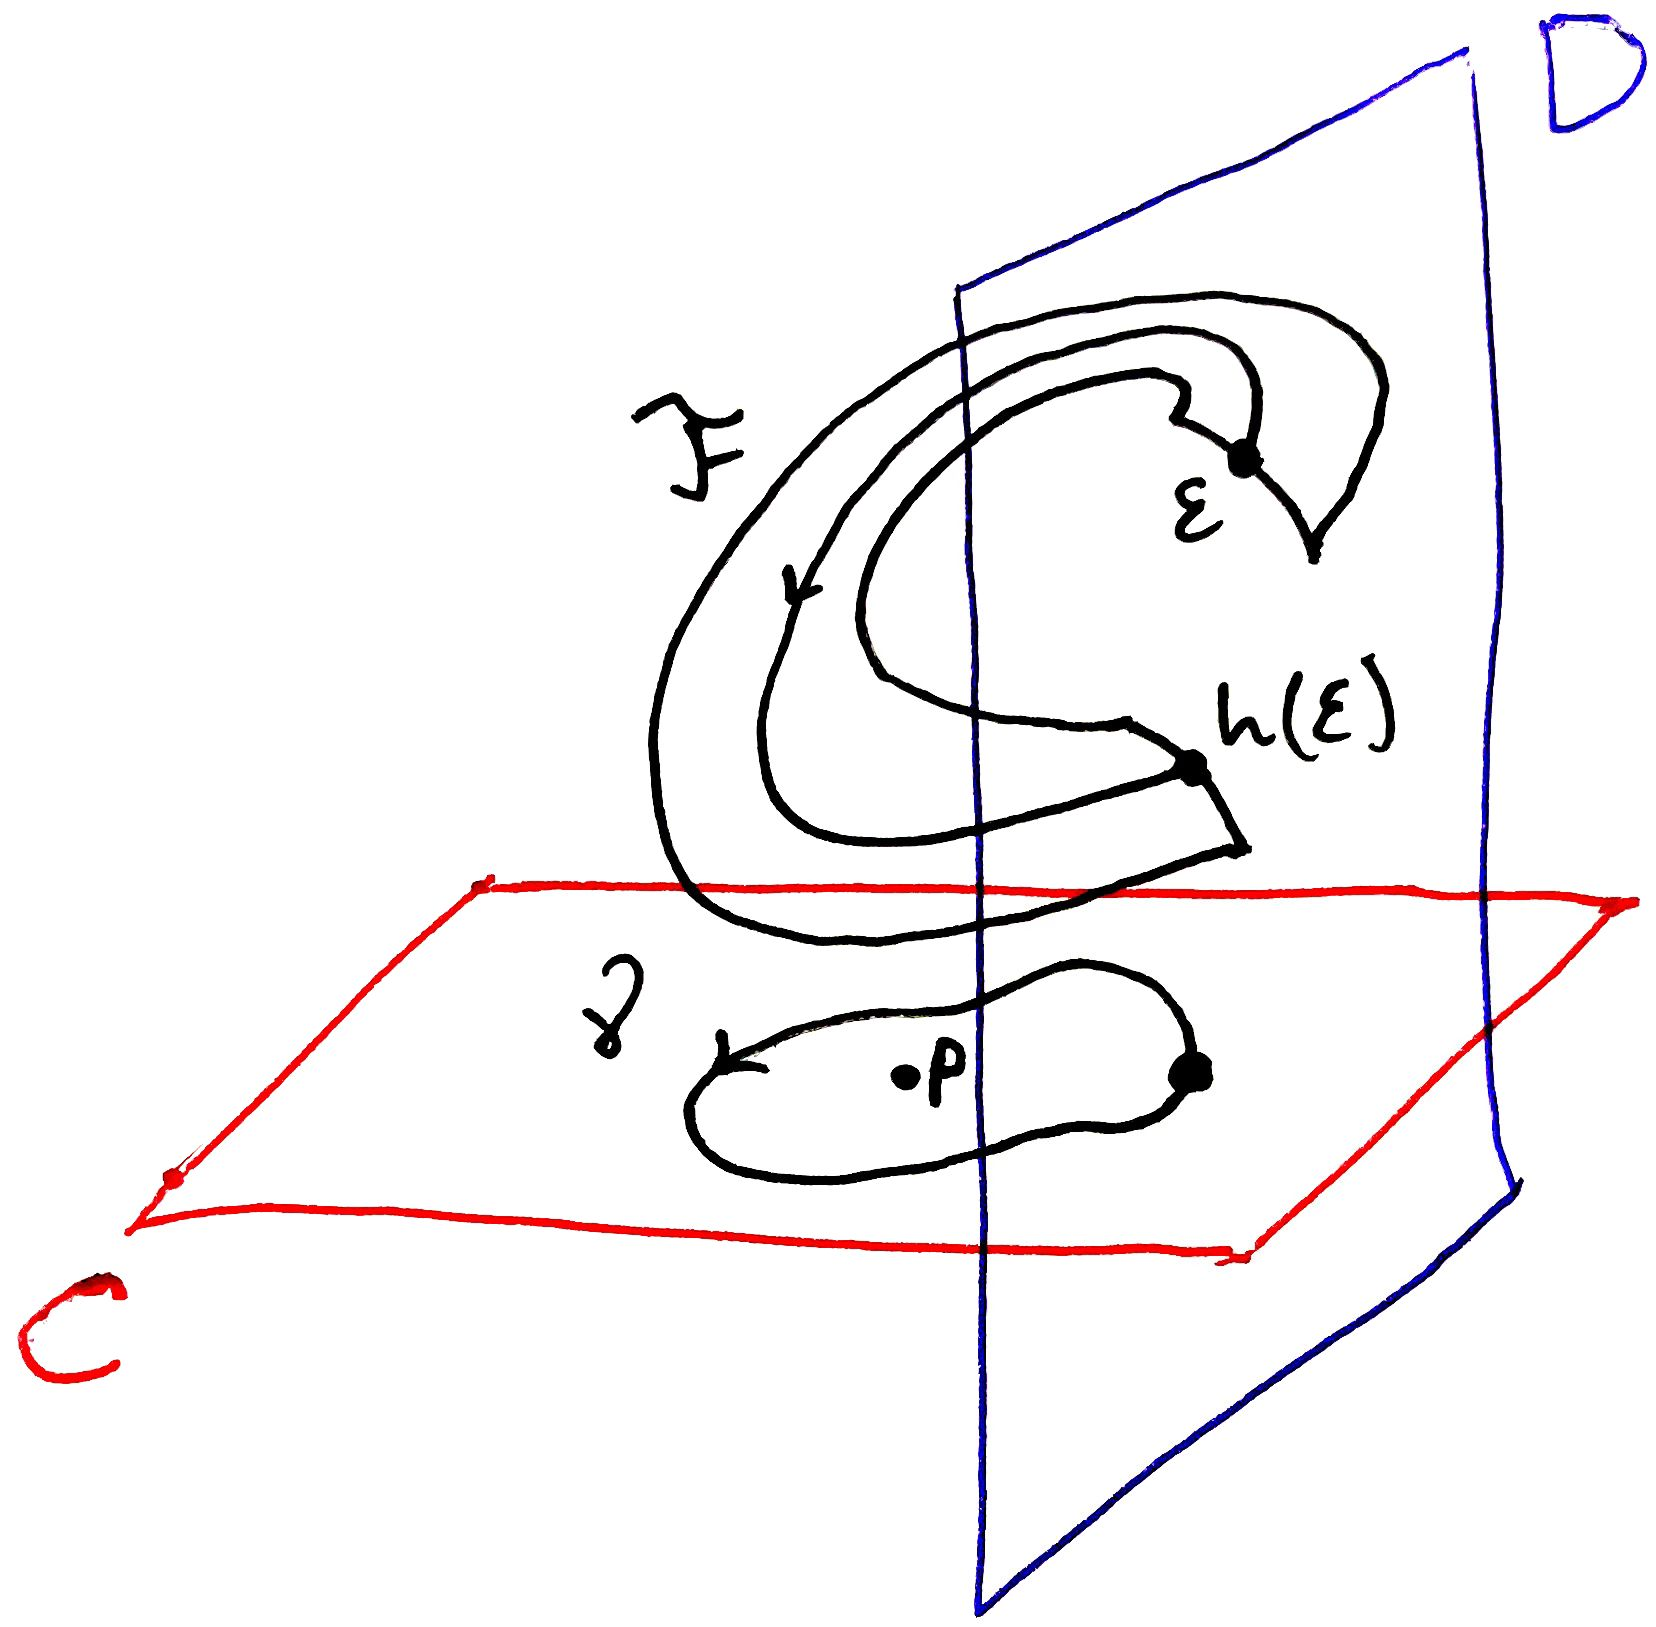
\includegraphics[scale=0.1]{holonomy}
    \caption{Holonomy of a foliation.}
\end{figure}

\begin{definition}
    The \emph{holonomy} of the separatrix $C$ is the (locally defined)
    biholomorphism of a disc neighbourhood of $p$ in $D$ coming from a generator
    of $\pi_1(C\setminus\{p\})$ with positive orientation, which is defined up
    to conjugacy. In practice we will only concern ourselves with the derivative
    of this (locally defined) biholomorphism at $p$, which is then a
    well-defined element of $\C^*$.
\end{definition}

To make things more concrete, suppose again that we have a local generator
$A\pdv{}{x}+B\pdv{}{y}$ for $\scrF$ near $p=(0,0)$, such that $C=\{y=0\}$. Take
$\gamma$ to be the loop $t\mapsto(e^{2\pi it},0)$ generating
$\pi_1(C\setminus\{p\})$. We have the projection $(x,y)\mapsto(x,0)\in C$, and
for each $\epsi\in\C$ we lift $\gamma$ to a path tangent to $\scrF$ starting at
$(1,\epsi)$ which has an endpoint $(1,h(\epsi))$. The holonomy is the map
$h(\epsi)$.

\begin{example}
    Consider the foliation generated by $x\pdv{}{x}+\lambda y\pdv{}{y}$. The
    leaves are locally fibers of the function $xy^{-\lambda}$, so lifting
    $(e^{2\pi it},0)$ to a path in the leaf through $(1,\epsi)$ we obtain
    $(e^{2\pi it},\epsi e^{2\pi i\lambda t})$, with endpoint
    $(1,\epsi e^{2\pi i\lambda})$. Hence we get
    $h(\epsi)=\epsi e^{2\pi i\lambda}$, so the holonomy of the separatrix
    $\{y=0\}$ is already linear with derivative $e^{2\pi i\lambda}$. Note that
    when $\lambda=-\sqrt2$ as in \cref{ex:irrational} this shows that the
    holonomy is an irrational rotation of infinite order, giving some evidence
    of the leaves not closing up nicely near the singularity.
\end{example}

\begin{example}\label{ex:radial holonomy}
    Consider the radial foliation generated by $x\pdv{}{x}+y\pdv{}{y}$. The leaf
    through $(1,\epsi)$ is the line it spans through the origin, and so lifting
    the loop $(e^{2\pi it},0)$ to this leaf gives
    $(e^{2\pi it},\epsi e^{2\pi it})$, which is again a loop. Hence the holonomy
    is trivial in this example.
\end{example}

The holonomy of a separatrix actually determines the local properties of $\scrF$
at the singularity in $p$ for certain classes of reduced singularities, due to
results in \cite{mattei_80}, \cite{martinet_82}.

\subsubsection{Eigenvalues}

Near a singularity, as in the study of dynamical systems, we can consider the
linearization of the generating vector field, replacing
\begin{equation*}
    A(x,y)\pdv{}{x} + B(x,y)\pdv{}{y}
\end{equation*}
with
\begin{equation*}
    \biggl(\pdv{A}{x}\bigg|_p\cdot x+\pdv{A}{y}\bigg|_p\cdot y\biggr)\pdv{}{x}
        + \biggl(\pdv{B}{x}\bigg|_p\cdot x+\pdv{B}{y}\bigg|_p\cdot y\biggr)
            \pdv{}{y}.
\end{equation*}
The resulting linear system is integrable, with integral curves given by
$t\mapsto e^{Jt}v_0$ for $J$ the Jacobian matrix of coefficients, so the salient
properties of the linearized dynamics are determined by the eigenvalues
$\lambda_1,\lambda_2$ of the matrix $J$, which is determined up to conjugation
by the choice of generating vector field.

\begin{definition}
    If $\lambda_1$ and $\lambda_2$ are not both zero, we say that
    $\lambda_1/\lambda_2$ if $\lambda_2\ne0$, or $\lambda_2/\lambda_1$ if
    $\lambda_1\ne0$, is the \emph{eigenvalue} of $\scrF$ at the singularity $p$,
    a complex number defined up to inversion. If the eigenvalue $\lambda$ is not
    a positive rational number, we say that the singularity is \emph{reduced}.
    If $\lambda\ne0$ we say the reduced singularity is \emph{non-degenerate},
    otherwise it is a \emph{saddle-node}.
\end{definition}

\begin{remark}
    Multiplication by a non-vanishing holomorphic function scales $\lambda_1$
    and $\lambda_2$ proportionally, so that the eigenvalue is well-defined up to
    inversion in terms of $\scrF$ and $p$. The concept of a reduced singularity
    of a foliation is well-defined since the positive rational numbers are
    closed under inversion.
\end{remark}

\begin{example}
    The radial foliation generated by $x\pdv{}{x}+y\pdv{}{y}$
    (\cref{fig:parallel}) has $\lambda=\lambda_1=\lambda_2=1$, and so the origin
    is not a reduced singularity. On the other hand, the foliation generated by
    $x\pdv{}{x}-\sqrt2y\pdv{}{y}$ (\cref{fig:irrational}) is reduced, with
    eigenvalue $-\sqrt2$. The singularity with positive multiplicity given
    by $x\pdv{}{x}+y^2\pdv{}{y}$ (\cref{fig:saddle-node}) is an example of a
    saddle-node.
\end{example}

In fact, reduced singularities have a classification with normal forms,
depending on the values of $\lambda$ (see \cite[\S1]{brunella_book}). A key
property of this classification is that the separatrices at a reduced
singularity form a local complete intersection, with at most 2 components.
Compare this with the non-reduced radial foliation of \cref{ex:parallel}, which
has infinitely many separatrices. The significance of this class of
singularities is that we can ``reduce'' to them after some sequence of blowups,
\cref{thm:seidenberg}, and moreover the blowup of a reduced singularity remains
reduced.

\subsection{Blowups}

\begin{example}\label{ex:blowup radial}
    Consider the foliation of $\P^2$ from \cref{ex:parallel}. In coordinates
    $[1:x:y]$ we have a singularity of the form $xdy-ydx$ with many
    separatrices, which we would like to blow up. Over this region, the blowup
    $X$ is covered by charts $U,V\simeq\A^2$ where
    $U=\{(x,tx,1:t)\in\A^2\times\P^1\}$, $V=\{(sy,y,s:1)\in\A^2\times\P^1\}$.
    The pullbacks to $U$ and $V$ of $\omega=zdy-ydz$ are
    \begin{equation*}
        \omega|_U = xd(tx)-txdx = x^2dt, \quad
        \omega|_V = sydy - yd(sy) = -y^2ds.
    \end{equation*}
    These vanish to second order along the exceptional divisor $E$, but
    factoring this out we get 1-forms $dt$ and $-ds$ on $U$ and $V$ which patch
    together to give a nowhere vanishing 1-form with values in the line bundle
    $\O(-2E)$. (Note that $dt=-ds/s^2$, $-ds=dt/t^2$.) Pictorially this is
    exactly as expected.
    \begin{figure}[H]
        \centering
        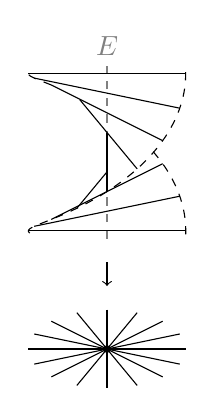
\begin{tikzpicture}
            \draw[color=gray,dashed] (0,0.9) -- (0,3.1)
                node[anchor=south] {$E$};

            \draw (1,1) -- (-1,1);
            \draw (0.924,1.441) -- (-0.924,1.059);
            \draw (0.707,1.854) -- (-0.707,1.146);
            \draw (0,1.75) -- (-0.383,1.288);
            \draw (0,2.25) -- (-0,1.5);
            \draw (-0.345,2.666) -- (0.383,1.788);
            \draw (-0.707,2.854) -- (0.707,2.146);
            \draw (-0.924,2.941) -- (0.924,2.559);
            \draw (-1,3) -- (1,3);

            \draw[domain=-0.1:2.4, dashed, smooth, variable=\t]
                plot ({cos(\t*22.5)}, {1+0.25*\t+0.5*sin(\t*22.5)});
            \draw[domain=6:8, dashed, smooth, variable=\t]
                plot ({cos(\t*22.5)}, {1+0.25*\t+0.5*sin(\t*22.5)});
            \draw[domain=-0.5:8.1, dashed, smooth, variable=\t]
                plot ({-cos(\t*22.5)}, {1+0.25*\t-0.5*sin(\t*22.5)});

            \draw[->] (0,0.6) -- (0,0.3);

            \draw (-1,-0.5)
                -- (0,-0.5) node[circle,fill,inner sep=1pt] {}
                -- (1,-0.5);
            \foreach \t in {1,...,7}
                \draw ({cos(\t*22.5)},{0.5*sin(\t*22.5)-0.5})
                    -- ({-cos(\t*22.5)},{-0.5*sin(\t*22.5)-0.5});
        \end{tikzpicture}
        \caption{Blowing up $xdy-ydx$.}
    \end{figure}
\end{example}

\begin{example}
    If we instead have the singularity $\omega=xdy+ydx$, then
    \begin{equation*}
        \omega|_U = x^2dt + 2xtdx, \quad
        \omega|_V = y^2ds+2ysdy.
    \end{equation*}
    This has only first order vanishing along $E$, giving a 1-form valued in
    $\O(-E)$, but with two singularities from the local forms $xdt+2tdx$,
    $yds+2sdy$. The exceptional divisor takes the role of the other separatrix
    downstairs in lifting the singularity.
    \begin{figure}[H]
        \centering
        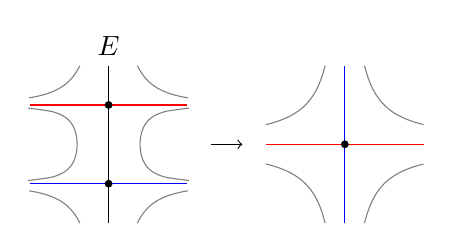
\begin{tikzpicture}
            \draw[color=blue] (-2,-0.5) -- (0,-0.5);
            \draw[color=red] (-2,0.5) -- (0,0.5);
            \draw (-1,-1) -- (-1,1) node[anchor=south] {$E$};
            \node[circle,fill,inner sep=1pt] at (-1,0.5) {};
            \node[circle,fill,inner sep=1pt] at (-1,-0.5) {};
            \foreach \s in {-1,1}
                \draw[domain=0.04:0.96, color=gray, smooth, variable=\t]
                    plot ({-1+\s*0.2/sqrt(\t*(1-\t))},{\t-0.5});
            \foreach \s in {-1,1}
                \draw[domain=1.09:1.5, color=gray, smooth, variable=\t]
                    plot ({-1+\s*sqrt(0.1/(\t*(\t-1)))},{\t-0.5});
            \foreach \s in {-1,1}
                \draw[domain=-0.5:-0.09, color=gray, smooth, variable=\t]
                    plot ({-1+\s*sqrt(0.1/(\t*(\t-1)))},{\t-0.5});

            \draw[->] (0.3,0) -- (0.7,0);

            \draw[color=blue] (2,-1) -- (2,1);
            \draw[color=red] (1,0) -- (3,0);
            \node[circle,fill,inner sep=1pt] at (2,0) {};
            \foreach \s in {-0.25,0.25}
                \draw[domain=-1:-0.25, color=gray, smooth, variable=\t]
                    plot ({2+\t}, {\s/\t});
            \foreach \s in {-0.25,0.25}
                \draw[domain=0.25:1, color=gray, smooth, variable=\t]
                    plot ({2+\t}, {\s/\t});
        \end{tikzpicture}
        \caption{Blowing up $xdy+ydx$.}
    \end{figure}
\end{example}

\begin{example}\label{ex:smooth blowup}
    Finally, consider blowing up a smooth foliation; $\omega=dx$. Then
    \begin{equation*}
        \omega|_U = dx, \quad \omega|_V = sdy+yds,
    \end{equation*}
    so we have introduced a singularity on the exceptional divisor, which
    crosses the strict transform of the unique separatrix downstairs. Note that
    the pullback doesn't vanish along $E$.
    \begin{figure}[H]
        \centering
        \begin{tikzpicture}
            \draw[color=red] (-2,-1) -- (-2,1) node[anchor=south] {$E$};
            \draw (-3,0) -- (-1,0);
            \node[circle,fill,inner sep=1pt] at (-2,0) {};
            \foreach \s in {-0.25,0.25}
                \draw[domain=-1:-0.25, color=gray, smooth, variable=\t]
                    plot ({-2+\t}, {\s/\t});
            \foreach \s in {-0.25,0.25}
                \draw[domain=0.25:1, color=gray, smooth, variable=\t]
                    plot ({-2+\t}, {\s/\t});

            \draw[->] (0,0) -- (0.5,0);

            \node[cross out,draw=black,inner sep=1pt] at (2,0) {};
            \draw (1,0) -- (3,0);
            \foreach \y in {-0.4,-0.2,0.2,0.4}
                \draw[color=gray] (1,{\y}) -- (3,{\y});
        \end{tikzpicture}
        \caption{Blowing up a smooth foliation.}
    \end{figure}
\end{example}

\begin{definition}
    Summarizing what we have seen in these examples, if $(X,\scrF)$ is a
    foliated surface and $p\in X$, then under the blowup
    $\pi:\tilde X=\Bl_pX\to X$ we have a rational section of
    $\pi^*N_\scrF\otimes\Omega^1_{\tilde X}$ with a zero of some order $a\ge0$
    along the exceptional divisor $E$. This then gives a regular section of
    $\pi^*N_\scrF(-aE)\otimes\Omega^1_{\tilde X}$, defining a foliation
    $\tilde\scrF$ on $\tilde X$ with $N_{\tilde\scrF}=\pi^*N_\scrF(-aE)$. We
    will refer to the vanishing order $a$ as $a(\scrF,p)$.
\end{definition}

\begin{remark}
    By a similar argument, we can pullback the foliation $\scrF$ along any
    rational map due to the characterization of foliations in terms of rational
    sections of $\Omega^1_X$, but in this generality we have less control over
    how the normal bundle changes.
\end{remark}

In \cref{ex:smooth blowup} we computed $a(\scrF,p)=0$ for
$p\notin\Sing(\scrF)$, and in the other examples we found $a(\scrF,p)=1$ for the
reduced singularity $xdy+ydx$ and $a(\scrF,p)=2$ for the non-reduced radial
singularity. It is a fact that for reduced singularities $a(\scrF,p)\in\{0,1\}$,
which can be shown from the normal forms. Recall that $K_{\tilde X}=K_X+E$, so
\begin{equation*}
    K_{\tilde\scrF}
        = K_{\tilde X}+N_{\tilde\scrF}
        = \pi^*K_\scrF+(1-a)E.
\end{equation*}
Hence for reduced singularities we get $K_{\tilde\scrF}\ge\pi^*K_\scrF$.

We now make a remark about the holonomy of the foliation $\tilde\scrF$. For each
separatrix $C$ through $p$, the strict transform $\tilde C\subset\tilde X$ is an
invariant curve of $\tilde\scrF$ that meets the exceptional divisor $E$ at a
point $q$, which may or may not be a singularity of $\tilde\scrF$.

\begin{proposition}\label{prop:blowup holonomy}
    The derivative of the holonomy of $\tilde\scrF$ along $\tilde C$ through $q$
    is the same as that of $\scrF$ along $C$ through $p$.
\end{proposition}

\begin{proof}
    Indeed, the loop $\gamma$, curve $D$, and portions of leaves along which
    $\gamma$ is lifted in the definition of the holonomy are all disjoint from
    $p$, and so lift isomorphically to the same constructions in $\tilde X$.
\end{proof}

\begin{example}
    In \cref{ex:radial holonomy} we saw that the radial fibration has trivial
    holonomy, which can be seen in light of this proposition from the fact that
    blowing it up gives a smooth foliation (\cref{ex:blowup radial}).
\end{example}

We conclude the section by citing Seidenberg's theorem on reduced singularities.

\begin{theorem}[Seidenberg, \cite{seidenberg_68}]\label{thm:seidenberg}
    If $(X,\scrF)$ is a foliated surface, and $p\in\Sing(\scrF)$, then there is
    a sequence of blowups $\pi:\tilde X\to X$ of centres over $p$ such that the
    induced foliation $\tilde\scrF$ has only reduced singularities on the fiber
    over $p$.
\end{theorem}

The basic idea of the proof is to keep track of multiplicities when blowing up,
allowing to pass to the case where the linearization is non-zero, and case
analysis of the vanishing orders along the exceptional divisors allows to
conclude. See \cite[\S1]{brunella_book} for details.
